%Dokumentklasse

%draft als optionohne bilder für bessere performance
%\documentclass[a4paper,12pt,]{scrreprt}

%normal mit Bildern
\documentclass[
a4paper,
11pt,
draft=True]
{scrartcl}

%Section als Chapter
\RedeclareSectionCommand[%
%beforeskip = -1sp plus -1sp minus -1sp,% kleinster negativer Wert, um den Absatzeinzug nach der Überschrift zu verhindern.
afterskip = 1.5 \baselineskip plus -1sp minus 1sp,
font = \Huge,
]{section}

\usepackage[left= 3cm,right = 3cm, bottom = 3cm,top = 3cm]{geometry}
%\usepackage[onehalfspacing]{setspace}

% ============= Packages =============
% Dokumentinformationen
\usepackage[
pdftitle={Praktikum - Umwelttechnik},
pdfsubject={},
pdfauthor={Roman-Luca Zank},
pdfkeywords={},	
%Links nicht einrahmen
hidelinks
]{hyperref}

%nur Text zum prüfen des Umfangs

% Standard Packages
%\usepackage[bottom]{footmisc}
\usepackage[utf8]{inputenc}
\usepackage[ngerman]{babel}

\usepackage[T1]{fontenc}
%\usepackage{helvet}

%\renewcommand{\familydefault}{\sfdefault}

\usepackage{graphicx}
\graphicspath{{img/}}
\usepackage{mhchem}
\usepackage{fancyhdr}
\usepackage{lmodern}
\usepackage{color}
\usepackage[bottom]{footmisc}
\usepackage{setspace}\usepackage{threeparttable}
%==================================================================
%\begin{threeparttable} 
%	\begin{tabular}{|l|c|r|} 
%		\hline 
%		A & B & C \\
%		\hline
%		1 & 2 & 3 \tnote{1} \\
%		\hline
%	\end{tabular} 
%	\begin{tablenotes}\footnotesize 
%		\item[1] Prognose 2003 
%	\end{tablenotes}
%====================================================================
\usepackage{placeins}
\usepackage{booktabs}
\usepackage{caption}
\usepackage[list=true]{subcaption}
\usepackage{longtable}
\usepackage{tikz}
\usepackage{pgfplots}
\usepackage{lastpage}
%\usepackage{ulem}
\usepackage{mathtools}
\usepackage{adjustbox}
\usetikzlibrary{patterns}
\usepackage{pdfpages}

%Einheitenpackage
\usepackage{siunitx}  
\sisetup{	locale = DE, 
	per-mode=fraction,
	inter-unit-product=\ensuremath{\cdot},
	detect-weight = true,
	quotient-mode=fraction
}
%neue Einheiten definieren
\DeclareSIUnit\xyz{xyz}	
\DeclareSIUnit\rpm{rpm}	
\DeclareSIUnit\mws{mWS}	
\DeclareSIUnit\degrees{^\circ}	

%Automatisch cdot statt *
\DeclareMathSymbol{*}{\mathbin}{symbols}{"01}


%Tabelle
\usepackage{tabularx}
\usepackage{tabulary}

%nur letzte Zeile der Gleichung nummerieren
\makeatletter
\def\Let@{\def\\{\notag\math@cr}}
\makeatother

% zusätzliche Schriftzeichen der American Mathematical Society
\usepackage{amsfonts}
\usepackage{amsmath}

%Abkürzungsverzeichnis
\usepackage{acronym}

%kein Abstand bei neuem Kapitel vom Seitenanfang
%\vspace*{2.3\baselineskip} = ORIGINAL
%\renewcommand*{\chapterheadstartvskip}{\vspace*{.0\baselineskip}}

%nicht einrücken nach Absatz
\setlength{\parindent}{0pt}

\urlstyle{same}


% ============= Kopf- und Fußzeile =============
\pagestyle{fancy}
%
\lhead{}
\chead{}
\rhead{}%\slshape }%\leftmark}
%%
\lfoot{}
\cfoot{}
\rfoot[{\thepage\ of \pageref*{LastPage}}]{Seite \thepage\ von \pageref*{LastPage}}
%%
\renewcommand{\headrulewidth}{0pt}
\renewcommand{\footrulewidth}{0pt}
%\renewcommand{\chapterpagestyle}{fancy}

%Fußnotelinie
%\let\footnoterule

%Fußnote mit Klammer
\renewcommand*{\thefootnote}{(\arabic{footnote})}

%Abb. statt Abbildung
\addto\captionsngerman{%
	\renewcommand{\figurename}{Abb.}%
	\renewcommand{\tablename}{Tab.}%
}

% ============= Package Einstellungen & Sonstiges ============= 
%Besondere Trennungen
%\hyphenation{De-zi-mal-tren-nung}
\usepackage[none]{hyphenat}
\hyphenpenalty=5000
\tolerance=5000
\providecommand\phantomsection{}

\usepackage{mathtools}


% ============= Dokumentbeginn =============

\begin{document}
%Seiten ohne Kopf- und Fußzeile sowie Seitenzahl
\pagestyle{empty}

%\begin{center}
\begin{tabular}{p{\textwidth}}


\begin{center}

\includegraphics[scale=0.75]{logos.jpg}\\
\end{center}


\\

\begin{center}
\LARGE{\textsc{
Protokoll \\
Analytik\\
}}
\end{center}

\\

%\begin{center}
%\large{Fakultät für Muster und Beispiele \\
%der Hochschule Musterhausen \\}
%\end{center}
%
%\\
\begin{center}
	\textbf{\LARGE{Versuch 1.5}}\\
	\vspace{5mm}
	\textbf{\Large{Redoxtitration}}

\end{center}
\begin{center}
\Large{Bestimmung des Wassergehalt von Flüssigkeiten und Feststoffen (Iodometrie)}
\end{center}

\begin{center}
	\large{Gruppe 2.4 (BCUC4)}
\end{center}


\\
%\begin{center}
%zur Erlangung des akademischen Grades\\
%Bachelor of Engineering
%\end{center}


%\begin{center}
%vorgelegt von
%\end{center}

\begin{center}
\Large{\textbf{Teilnehmer:}} \\ 
\end{center}
\begin{center}
\large{Willy Messerschmidt \\
	Roman-Luca Zank} \\
\end{center}


\\

\begin{center}
\begin{tabular}{lll}
%\large{\textbf{Protokollführer:}} & & \large{NAME}\\
&&\\
\large{\textbf{Datum der Versuchsdurchführung:}}&& \large{29.05.2020 (Online)}\\
&&\\
\large{\textbf{Abgabedatum:}}&& \large{12.06.2020}
\end{tabular}
\end{center}

\\ \\ \\ \\ \\ \\ \\ \\ 
\large{Merseburg den \today}

\end{tabular}
\end{center}


%\include{14_danksagungen}

%\include{15_zusammenfassung}

% Beendet eine Seite und erzwingt auf den nachfolgenden Seiten die Ausgabe aller Gleitobjekte (z.B. Abbildungen), die bislang definiert, aber noch nicht ausgegeben wurden. Dieser Befehl fügt, falls nötig, eine leere Seite ein, sodaß die nächste Seite nach den Gleitobjekten eine ungerade Seitennummer hat. 
\cleardoubleoddpage

% Pagestyle für Titelblatt leer
\pagestyle{empty}

%Seite zählen ab
\setcounter{page}{0}

%Titelblatt
\begin{center}
\begin{tabular}{p{\textwidth}}


\begin{center}

\includegraphics[scale=0.75]{logos.jpg}\\
\end{center}


\\

\begin{center}
\LARGE{\textsc{
Protokoll \\
Analytik\\
}}
\end{center}

\\

%\begin{center}
%\large{Fakultät für Muster und Beispiele \\
%der Hochschule Musterhausen \\}
%\end{center}
%
%\\
\begin{center}
	\textbf{\LARGE{Versuch 1.5}}\\
	\vspace{5mm}
	\textbf{\Large{Redoxtitration}}

\end{center}
\begin{center}
\Large{Bestimmung des Wassergehalt von Flüssigkeiten und Feststoffen (Iodometrie)}
\end{center}

\begin{center}
	\large{Gruppe 2.4 (BCUC4)}
\end{center}


\\
%\begin{center}
%zur Erlangung des akademischen Grades\\
%Bachelor of Engineering
%\end{center}


%\begin{center}
%vorgelegt von
%\end{center}

\begin{center}
\Large{\textbf{Teilnehmer:}} \\ 
\end{center}
\begin{center}
\large{Willy Messerschmidt \\
	Roman-Luca Zank} \\
\end{center}


\\

\begin{center}
\begin{tabular}{lll}
%\large{\textbf{Protokollführer:}} & & \large{NAME}\\
&&\\
\large{\textbf{Datum der Versuchsdurchführung:}}&& \large{29.05.2020 (Online)}\\
&&\\
\large{\textbf{Abgabedatum:}}&& \large{12.06.2020}
\end{tabular}
\end{center}

\\ \\ \\ \\ \\ \\ \\ \\ 
\large{Merseburg den \today}

\end{tabular}
\end{center}
 %Prokolle
%\begin{center}
\begin{tabular}{p{\textwidth}}


\begin{center}

\includegraphics[scale=0.75]{img/logos.jpg}\\
\end{center}


\\

\begin{center}
\LARGE{\textsc{
Recherche \\
Rückgewinnung von Ammoniak aus Industrieabwässern\\
}}
\end{center}

%\begin{center}
%\large{Fakultät für Muster und Beispiele \\
%der Hochschule Musterhausen \\}
%\end{center}
%
%\\
 \\
 
\begin{center}
\textbf{\Large{Seminararbeit in Medienrecherche}}
\end{center}

\begin{center}
	\large{im WiSe 2019}
\end{center}
 \\
%\begin{center}
%zur Erlangung des akademischen Grades\\
%Bachelor of Engineering
%\end{center}


\begin{center}
\large{vorgelegt von}
\end{center}
\\


\begin{center}
\Large{\textbf{Roman-Luca Zank}} \\
\end{center}

\begin{center}
3. Semester \\
Chemie- und Umwelttechnik \\
\end{center}


\begin{center}
\begin{tabular}{lll}
	\textbf{E-Mail:} & & romanzank@mail.de\\
	\textbf{Matrikelnummer:} & &25240\\
	\textbf{Adresse:} & &Platz der Bausoldaten 2, Zimmer 224\\
	\textbf{Ort:} & &06217 Merseburg\\
	&& \\
	\textbf{Prüfer:} & & Dr. Frank  Baumann\\
\end{tabular}
\end{center}

\\ \\ \\ \\ \\
\large{Merseburg, \today}

\end{tabular}
\end{center}
 %Seminar-/Abschlussarbeit

% Pagestyle für Rest des Dokuments
\pagestyle{fancy}

%Inhaltsverzeichnis
\tableofcontents
\thispagestyle{empty}

%Inhalt
%
%Verzeichnis aller Bilder
\label{sec:bilder}
\listoffigures
\addcontentsline{toc}{chapter}{Abbildungsverzeichnis}
\thispagestyle{empty}

%Verzeichnis aller Tabellen
\label{sec:tabellen}
\listoftables
\addcontentsline{toc}{chapter}{Tabellenverzeichnis}
\thispagestyle{empty}



%%Abkürzungsverzeichnis
%\setlength{\columnsep}{20pt}
%\twocolumn
%\addchap{Nomenklatur}
%\label{sec:abkurzung}
%\begin{acronym}
%\acro{kf}[$\text{k}_\text{f}$]{Durchlässigkeitsbeiwert}
%\acro{t}{Durchlaufzeit}
%\acro{tm}[$\text{t}_\text{m}$]{Mittlere Durchlaufzeit}
%\acro{V}{Volumen}
%\acro{h}{Höhe der Wassersäule}
%\acro{Q}{Volumenstrom}
%\acro{l}{Durchströmte Länge}
%\acro{A}{Grundfläche}
%\acro{d}{Durchmesser}
%
%\end{acronym}
%\subsubsection{Aufrufen einer Abkürzung}
%\acs{rT}
%\begin{verbatim}
%\acs{Abkürzung}
%\end{verbatim}

%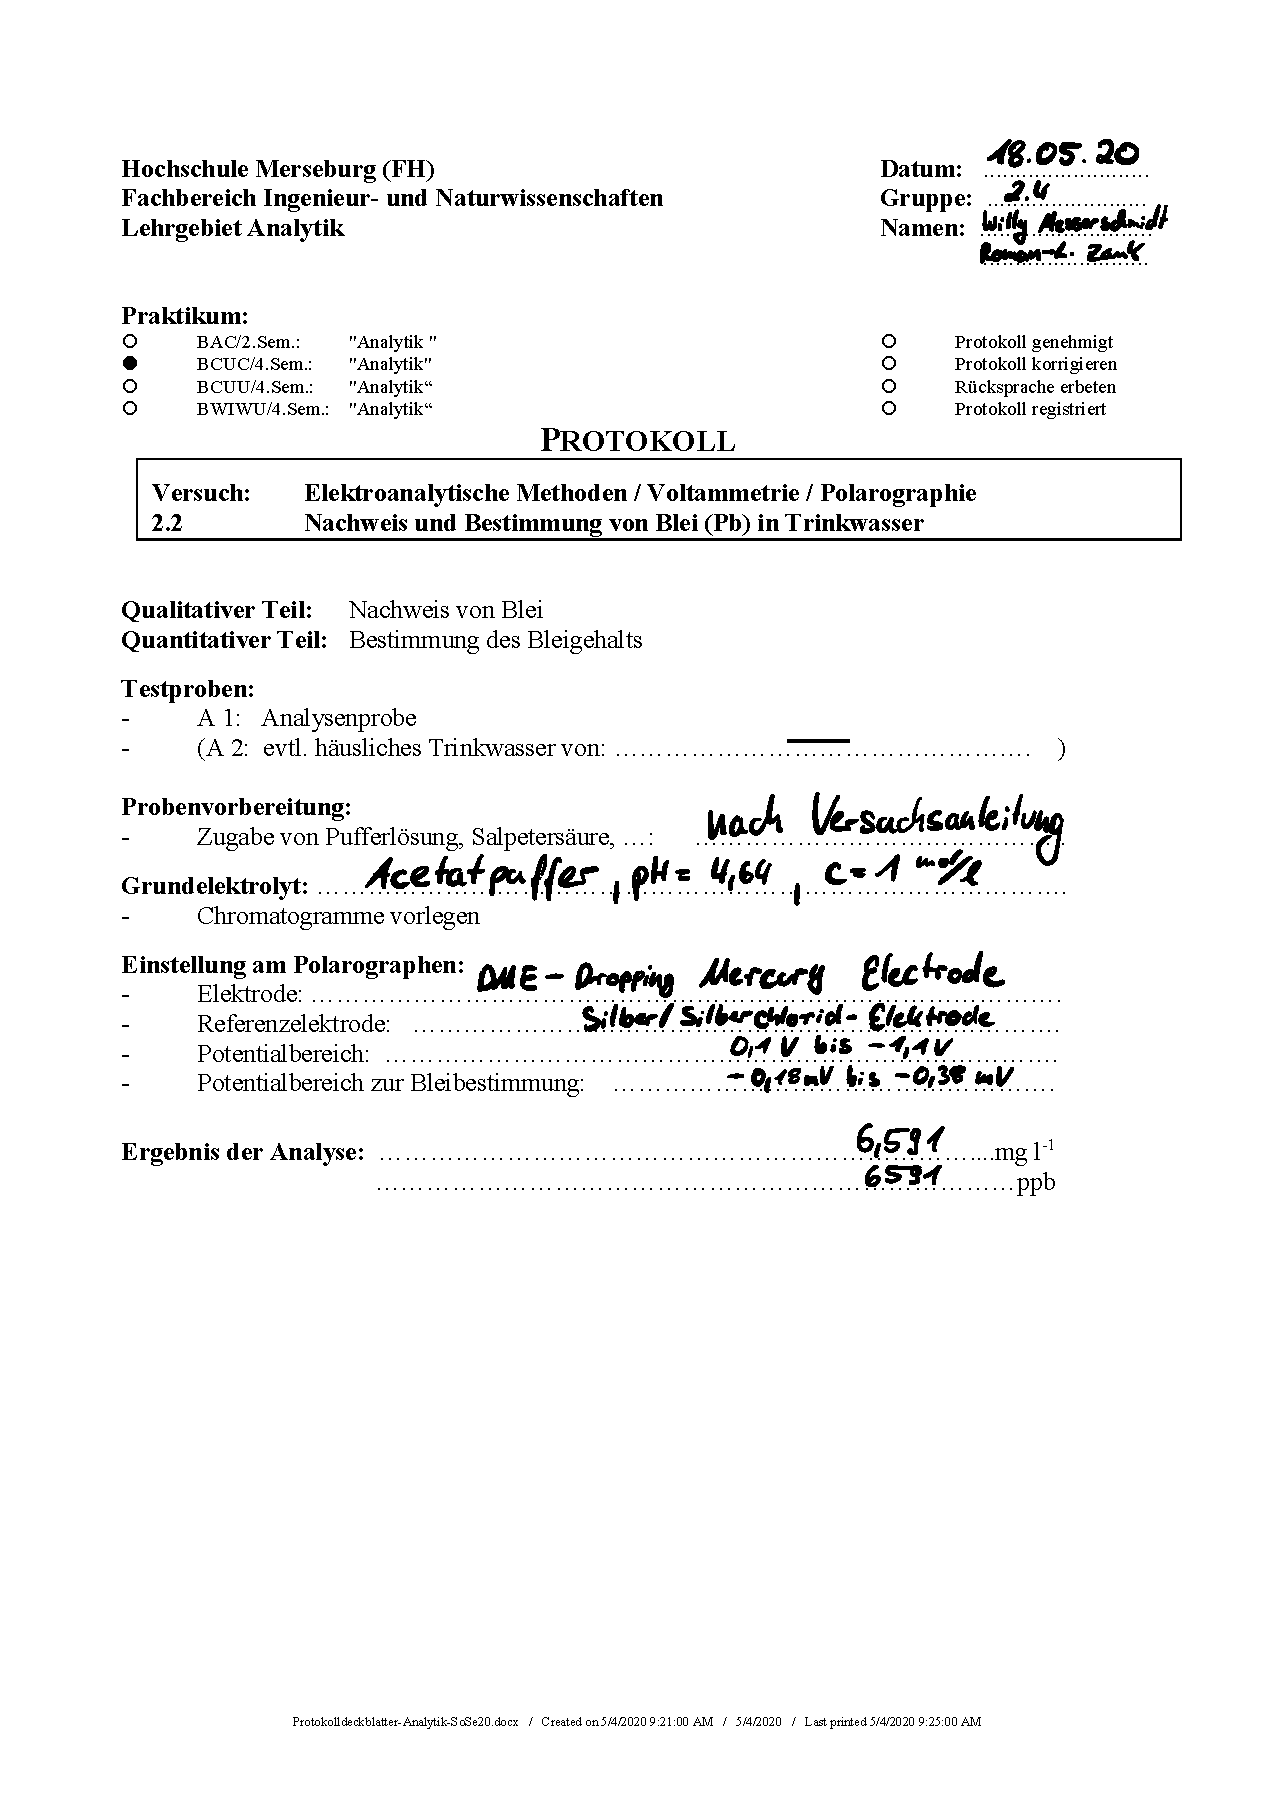
\includepdf[]{Deckblatt}
\pagebreak
\section{Einleitung}
\label{sec:einleitung}
Ein hoher Chloridgehalt im Trink-, sowie Brauchwasser kann aufgrund von Geschmacksbeeinträchtigung bei der Herstellung von Getränken wie Tee oder Kaffee unerwünscht sein. Für eisenhaltige Metalle können zu hohe Chloridgehalte sogar korrosiv wirken. Die Herkunft von erhöhten Chloridgehalten können in Abwässern, Düngemitteln oder auch Fäkalien liegen. Unter der Voraussetzung, dass das Trinkwasser nicht korrosiv wirken sollte, gilt es, laut Trinkwasserverordnung, einen Grenzwert von \SI{250}{\milli \gram \per \liter} Chlorid einzuhalten.\\
Im Praktikum wird eine Leitungswasserprobe mittels Argentometrie auf diesen Grenzwert untersucht. Für die Titration werden die Messmethoden der Konduktometrie und Potentiometrie angewandt. Im Protokoll sind dabei verschiedene Methoden für Äquivalenzpunktbestimmung darzustellen. 






\section{Theorie}
\label{sec:theorie}

\textbf{\textcolor{red}{Aufgaben:}}
\textcolor{red}{
	\begin{itemize}
		\item In welche Kategorie fällt das Ammonium ? Ist es farbig ? Warum ?
		\item Verdünnungsrechnung
		\item Aufpassen bei Konzentrationsangaben wegen Runden
	\end{itemize}
}

\subsection{Labert-Beer'sches Gesetz}


\newpage
\section{Geräte und Chemikalien}
\label{sec:geraete}

\textbf{Geräte:}
\begin{itemize}
\item Vollpipetten (V=\SI{50}{\milli \liter } \& \SI{100}{\milli \liter } )
\item Bechergläser
\item Rührfisch mit Magnetrührer
\item Konduktometer mit Leitfähigkeitselektrode
\item pH-Meter mit Silber-Einstabmesskette (\textsc{Microprocessor pH 539})
\item Elektronische Bürette \textsc{Titronic 97/20}
\end{itemize}

\vspace*{5mm}

\textbf{Proben/Chemikalien:}
\begin{itemize}
\item Leitungswasserprobe
\item Destilliertes Wasser
\item Silbernitratlösung $\left(c=\SI{0,01}{\mol \per \liter}\right)$
\end{itemize}







\section{Durchführung}
\label{sec:durchfuerung}

Der Versuch begann mit dem Einschalten der elektronischen Bürette und des Leitfähigkeitsmessgerätes. Es wurde ohne Temperaturkorrektur durch das Messgerät gearbeitet. Die Messsonde wurde mit destilliertem Wasser gespült und in das Stativ eingespannt. Die Einstellungen an der elektronischen Bürette wurden beibehalten. An dieser Stelle wurden mittels einer Vollpipette exakt \SI{100}{\milli\liter} der Wasserprobe abgemessen und zusammen mit einem Rührfisch in ein Becherglas mit einem Volumen von \SI{125}{\milli\liter} eingefüllt. Das Becherglas wurde auf dem Magnetrührer platziert und die Elektrode herabgesenkt bis selbige ausreichend in die Lösung eingetaucht war. Es ist wichtig dass über dem Rührfisch genügend Raum bleibt um die Sonde gut eintauchen zu können. Das Drücken der Start-Taste an der elektronischen Bürette startet die Zugabe der 0,01 molaren Silbernitratlösung. Diese wird durch die automatische Bürette alle 15 Sekunden in Portionen von \SI{0,5}{\milli\liter} zugegeben, bis ein Gesamtvolumen von \SI{20}{\milli\liter} eingebracht wurde. Nach dem Einspritzen der Silbernitratlösung wurde immer 10 Sekunden gewartet, bis der Messwert vom Messgerät abgelesen wurde. Dieser Ablauf wurde 3 mal wiederholt, wobei für jede neue Wasserprobe ein frisches Becherglas genutzt wurde. Dann erfolgte der Wechsel von Sonde und Messgerät. Die Leitfähigkeitssonde wurde gespült und wieder in destilliertes Wasser getaucht, während die Silber-Silberchlorid-Elektrode als Einstabmesskette in das Stativ eingespannt wurde. Das Leitfähigkeitsmessgerät wurde aus- und das pH-Meter zur Messung der Potentialdifferenz eingeschaltet. Für die Potentiometrische Indikation wurden je nur \SI{50}{\milli\liter} Wasserprobe abgemessen. Da die Elektrode  nicht vom rotierenden Rührfisch getroffen werden darf und die Silberelektrode doch bis über das innen-liegende Diaphragma eingetaucht sein muss, wurden auch entsprechend kleinere Bechergläser genutzt. Aus den vorangegangenen konduktometrischen Messungen konnte geschlossen werden, das der Äquivalenzpunkt bei etwa \SI{3,5}{\milli\liter} Silbernitratlösung zu erwarten war. Die insgesamt zutitrierte Menge wurde daher an der elektronischen Bürette von den zuvor \SI{20}{\milli\liter}, auf \SI{10}{\milli\liter} herabgesetzt. Dies geht mit einer großen Zeitersparnis und der Einsparung von Chemikalien einher. Wiederum wurden die Werte nach 10 Sekunden abgelesen und notiert. Auch diesmal wurde eine Dreifachbestimmung vorgenommen.

Nach Abschluss der Messungen wurden alle silberhaltigen Abfälle in einen Sammelbehälter entsorgt und die Geräte abgewaschen. Die Silberelektrode wurde, wie die Leitfähikeitssonde auch, in ein Becherglas mit destilliertem Wasser gehangen um dem Austrocknen vorzubeugen.

Eine Bestimmung des Korrekturfaktors musste aus Zeitgründen entfallen.

\newpage

\vspace*{10mm}

\textbf{\textcolor{red}{Aufgaben:}}
\textcolor{red}{
	\begin{itemize}
		\item Verdünnungsrechnung
		\item Aufpassen bei Konzentrationsangaben wegen Runden
	\end{itemize}
}

\section{Ergebnisse und Berechnungen}
\label{sec:ergebnisse}


\textbf{Berechnung des Mittelwertes:}
\begin{flalign}
\label{Gl:Mittelwert-Beispielrechnung1}
\bar{x} &= \frac{\sum_{n=1}^{N}x_n}{N}\\ 
%\label{Gl:Mittelwert-Beispielrechnung2}
\bar{x} &= \frac{0,02+0,017+0,021}{3}\\
&= \underline{0,019}
\end{flalign}

\textbf{Berechnung der Standardabweichung:}
\begin{flalign}\label{Gl:Standardabweichung-Beispielrechnung}
s &= \sqrt{\frac{\sum_{n=1}^{N}(x_n-\bar{x})^2}{N-1}}
\end{flalign}
%	\begin{footnotesize}
\begin{flalign}
s &= \sqrt{\frac{(0,594\si{\milli\gram\per\liter}-0,694\si{\milli\gram\per\liter})^2+(0,914\si{\milli\gram\per\liter}-0,694\si{\milli\gram\per\liter})^2+(0,575\si{\milli\gram\per\liter}-0,694\si{\milli\gram\per\liter})^2}{2}}\\
&= \underline{0,19\si{\milli\gram\per\liter}}
\end{flalign}
%	\end{footnotesize}

\textbf{Berechnung der relativen Standardabweichung:}

\begin{flalign}\label{gl:S_rel}
	s_{rel}&=\frac{s}{\bar{x}}\\
	&=\frac{\SI{0,19}{\milli\gram\per\liter}}{\SI{0,69}{\milli\gram\per\liter}}\\
	&=\underline{28\%}
\end{flalign}

\textbf{Berechnung des Vertrauensintervalls:}\\
\begin{flalign}
conf(\bar{x}) 	&= \bar{x}\pm \frac{t}{\sqrt{N}}*s				
\end{flalign}
\begin{flalign}
conf(\bar{x})	&= \SI{0,0407}{\percent}\pm \frac{3,182}{\sqrt{4}}*\SI{0,0030}{\percent}\\
&= \underline{\SI{0,0407}{\percent}\pm \SI{0,0048}{\percent}}
\end{flalign}

\textbf{Manuelle Bestimmung des Wassergehaltes:}\\
Beispielhaft wird nachfolgend in Gleichung (\ref{gl:wassergehalt}) die manuelle Berechnung des Wassergehaltes der flüssigen Probe Isopropanol dargestellt. Dazu wurden Messwerte der Tabelle \ref{tab:MesswerteIsopropanol} für die Berechnung verwendet. Für den Titer wurde der Mittelwert aus Tabelle \ref{tab:MesswerteTiterbestimmung} genutzt.
%Aus dem Vorgängerprotokoll___Eiheiten sind totaler schwachsinn!
%\begin{flalign}\label{gl:wassergehalt}
%	Wassergehalt &= \frac{V_{EQ}*f+DriftV*t}{m_{Probe}}\\
%	&= \frac{\SI{0,00925}{\milli\liter}*1,045+\SI{5,5}{\micro\liter\per\minute}*\SI{1,18}{\minute}}{\SI{0,4037}{\gram}}\\
%\end{flalign}

\begin{flalign}\label{gl:wassergehalt}
	W [\%]&=\frac{(V_{EQ}+t*DRIFTV)*\bar{c}+DRIFT*t}{m_{Probe}}\\[2mm]
	&=\frac{(\SI{0,00925}{\milli\liter}+\SI{1,18}{\minute}*\SI{5,5}{\micro\liter\per\minute})*\SI{5,22732}{\milli\gram\per\milli\liter}
		+\SI{28,6}{\micro\gram\per\minute}*\SI{1,18}{\minute}}{\SI{0,4037}{\gram}}*100\%\\
	&=\underline{\underline{0,029\%}}
\end{flalign}

\newpage
\section{Diskussion}
\label{sec:diskussion}

%Aus den  Daten der konduktometrischen Indikation konnten die Reaktions- und Überschussgerade (siehe Abb. \ref{dia:kondukto}) mit einem Bestimmtheitsmaß von mindestens 0,999 \mbox{ (vgl. Tab. \ref{tab:konduk_regress}) }erhalten werden. Deren Schnittpunkt erlaubt, durch Fällung des Lotes auf die Abzisse, das Ablesen des Äquivalenzvolumens. In diesem Falle wurde das Äquivalenzvolumen aber berechnet (vgl. Gl. \eqref{Gl:KonduAEQV}). Es ergibt sich dafür im Mittel \SI{7,120}{\milli\liter} für \SI{100}{\milli\liter} der Wasserprobe. 
%
%Aus den Daten der potentiometrischen Indikation wurde der Äquivalenzpunkt durch das numerische Verfahren nach \textsc{Kolthoff-Hahn } bestimmt (vgl. Gl. \eqref{eq:kolthoff-hahn}). Für das Probenvolumen von \SI{50}{\milli\liter} wurde ein mittleres Äquivalenzvolumen von  \SI{3,66}{\milli \liter} ermittelt. Die Messdaten sind in Abb. \ref{dia:potentio} graphisch aufbereitet. Es fällt auf, dass die Messpunkte im unteren Bereich etwas weiter streuen. Die Ursache dafür wird beim Messgerät vermutet, da die relative Abweichung um einen konstanten Messfehler sich bei niedrigen Potentialen deutlich stärker auswirkt. 
%
%Die drei Messreihen liegen sowohl bei der Konduktometrie als auch bei der Potentiometrie sehr nah beieinander. Die Messungen sind daher präzise und wiederholgenau.

Aus den  Daten der konduktometrischen Indikation konnten die Reaktions- und Überschussgerade (siehe Abb. \ref{dia:kondukto}) mit einem Bestimmtheitsmaß von mindestens 0,999 \mbox{ (vgl. Tab. \ref{tab:konduk_regress})} erhalten werden. Deren Schnittpunkt erlaubt, durch Fällung des Lotes auf die Abzisse, das Ablesen des verbrauchten Volumens an Maßlösung. In diesem Falle wurde das Äquivalenzvolumen aber berechnet (vgl. Gl.\eqref{Gl:KonduAEQV}). Es ergibt sich dafür im Mittel \SI{7,120}{\milli\liter} für \SI{100}{\milli\liter} der Wasserprobe. 

Aus den Daten der potentiometrischen Indikation wurde der Äquivalenzpunkt durch das numerische Verfahren nach \textsc{Kolthoff-Hahn} bestimmt (vgl. Gl. \eqref{eq:kolthoff-hahn}). Für das Probenvolumen von \SI{50}{\milli\liter} wurde ein mittleres Äquivalenzvolumen von \SI{3,656}{\milli\liter} für \SI{100}{\milli\liter} erhalten. Zur besseren Vergleichbarkeit lässt sich dieses auf ein Probenvolumen von \SI{100}{\milli\liter} umrechnen. Für \SI{100}{\milli\liter} ergibt sich ein Äquivalenzvolumen von \SI{7,312}{\milli\liter}. Die Messdaten der potentiometrischen Indikation sind in Abb. \ref{dia:potentio} graphisch aufbereitet. Es fällt auf, dass die Messpunkte im unteren Bereich etwas weiter streuen. Die Ursache dafür wird beim Messgerät vermutet, da sich die relative Abweichung um einen konstanten Messfehler, bei niedrigen Potentialen deutlich stärker auswirkt. 


Aus den Äquivalenzvolumina kann, wie in Gl. \eqref{Gl:Chloridgehalt} dargestellt, der Chloridgehalt der untersuchten Wasserprobe berechnet werden. Die Mittelwerte des Chloridgehaltes liegen bei \SI{25,243}{\milli\gram\per\liter} und \SI{25,926}{\milli\gram\per\liter}. 




Die Einhaltung des Grenzwertes für Chlorid im Trinkwasser von \SI{250}{\milli\gram\per\liter}, wird durch einen Grenzwerttest bewiesen. 








Die drei Messreihen liegen, wie in den Abbildungen \ref{dia:kondukto} und \ref{dia:potentio} zu sehen ist, sowohl bei der Konduktometrie als auch bei der Potentiometrie, sehr nah bei einander. Die Messungen sind daher äußerst präzise und wiederholgenau. Dafür sprechen auch die relativen Standardabweichungen von nur rund 0,002. Die berechneten Chloridgehalte weichen nur um 1,5\% voneinander ab. 
Damit erweisen sich sowohl die konduktometrische, als auch die potentiometrische Indikation als gut geeignet um den Äquivalenzpunkt bei argentometrischen Untersuchungen anzuzeigen.



\section{Fehlerbetrachtung}
\label{sec:fehler}

Die Fehler in diesem Versuch werden hauptsächlich in Verunreinigungen vermutet. So wurden die Bechergläser vor dem Befüllen nicht noch einmal gespült und die Vollpipetten nur mit deionisiertem Wasser und nicht mit der Probe gespült. Die Messung könnte durch Staubpartikel aus der Luft in und an den Küvetten sowie im Photometer verfälscht worden sein. Es wurde für alle Messungen die gleiche Küvette genutzt. Das schließt den individuellen Einfluss der Wandungsbeschaffenheit als mögliche Fehlerquelle aus. 

Neben Verunreinigungen kann sich auch der unterschiedliche Verlauf der Komplexierungsreaktion der Ammoniumionen und störender Metallionen in den Ergebnissen niederschlagen. Bei der Probenvorbereitung wurden nicht alle Proben gleich behandelt. Manche Bechergläser wurden öfter als andere Verschoben. Diese unabsichtlich herbeigeführte Agitation der Lösungen könnte sich auf die darin ablaufenden Reaktionen ausgewirkt haben. 

Bei der Probenvorbereitung gehen außerdem die Toleranzen der Pipetten und Maßkolben als Fehler in das Experiment ein. 

Es konnte eine Erklärung für die auffällige Abweichung der Konzentration bei der zweiten Wiederholung der Messung der Analysenprobe A1 ausgemacht werden. Die Pipettierung der Analysenprobe A1 erfolgte \underline{nach} der Pipettierung der Probe A2. Aus der Versuchsauswertung geht hervor, dass die Probe A2 die höchst-konzentrierte ist. Es wird vermutet dass Rückstände an der Vollpipette zu einer Erhöhung des besagten Wertes beitrugen.


%\section*{Anhang}
\addcontentsline{toc}{section}{Anhang}
%\label{sec:anhang}
 
 
 
 

%Praktikumsskript, Modul ………, Versuch …….., Prof. Musterprof. 
%DIN 12345, Jahr der Veröffentlichung 
%Link der Internetseite, Zugriffsdatum 
%Buchtitel, Autor, Verlag, Veröffentlichungsjahr 

%Literaturverzeichnis Bücher
\bibliography{Literatur}
\bibliographystyle{unsrtdin}
\addcontentsline{toc}{section}{Literaturverzeichnis}



%\chapter*{Eidesstattliche Erklärung}
\label{erklaerung}
Hiermit versichere ich, die vorliegende Seminararbeit selbstständig und nur unter Verwendung der von mir angegebenen Quellen und Hilfsmittel verfasst zu haben. Sowohl inhaltlich als auch wörtlich entnommene Inhalte wurden als solche kenntlich gemacht. Die Arbeit hat in dieser oder vergleichbarer Form noch keinem anderem Prüfungsgremium vorgelegen. \\
\\[1.5cm]
Datum:	\hrulefill\enspace Unterschrift: \hrulefill
\\[3.5cm]
\addcontentsline{toc}{chapter}{Selbstständigkeitserklärung}

\end{document}
